\documentclass[a4paper,conference]{IEEEtran}
\IEEEoverridecommandlockouts
\usepackage{cite}
\usepackage{amsmath,amssymb,amsfonts}
\usepackage{graphicx}
\usepackage{textcomp}
\usepackage{xcolor}
\usepackage{booktabs}
\usepackage{multirow}
\usepackage{url}
\usepackage{microtype}
\usepackage{fontspec}
\setmainfont{TeX Gyre Termes}
\renewcommand{\IEEEkeywordsname}{Keywords}

\title{CropLens AI: APMC Market Intelligence, Supply Shock Detection \& Procurement Intelligence Platform}

\author{
    \IEEEauthorblockN{Krishan Kant Jha}
    \IEEEauthorblockA{
        \textit{Department of Information Technology}\\
        \textit{ABES Engineering College}\\
        Ghaziabad, India\\
        krishankant4019@gmail.com
    }
    \and
    \IEEEauthorblockN{Hemant Raghav}
    \IEEEauthorblockA{
        \textit{Department of Information Technology}\\
        \textit{ABES Engineering College}\\
        Ghaziabad, India\\
        hr246740@gmail.com
    }
    \and
    \IEEEauthorblockN{Divya Parashar}
    \IEEEauthorblockA{
        \textit{Department of Information Technology}\\
        \textit{ABES Engineering College}\\
        Ghaziabad, India\\
        parashardivy@gmail.com
    }
    \and
    \IEEEauthorblockN{Lokendra Sachan}
    \IEEEauthorblockA{
        \textit{Department of Information Technology}\\
        \textit{ABES Engineering College}\\
        Ghaziabad, India\\
        lokendrasachan20@gmail.com
    }
}

\begin{document}
\maketitle

\begin{abstract}
Many farmers and buyers in India's Agricultural Produce Market Committee (APMC) mandis must decide when and where to trade before tomorrow's wholesale price is known. A point forecast on its own hides how bad a price drop could be for a perishable crop, or how much budget risk a procurement plan carries. CropLens AI is a next-day price-forecasting and market-intelligence system built for this timing gap. It joins Agmarknet prices and arrivals with weather, Sentinel-2 NDVI, calendar, and spatial variables under a fixed 47-feature contract, and predicts next-day modal price for each commodity--mandi series. The historical panel from 2019--2025 is split chronologically, with 2019--2023 for training, 2024 for validation, and the full 2025 period held out for testing. The production model is a three-quantile LightGBM system (P10, P50, P90) with monotonic rearrangement and validation-only Conformalized Quantile Regression (CQR), benchmarked against Ridge, XGBoost, CatBoost, naive persistence, LSTM, GRU, Temporal Fusion Transformer, and a separate ARIMA(1,1,1) series baseline. On the frozen 2025 test set (19{,}240 rows), Ridge gives the lowest multivariate point error (MAE INR~56.58/qtl), while the ARIMA(1,1,1) protocol reaches MAE INR~48.04/qtl on its own series-level evaluation. The LightGBM band attains 79.49\% empirical coverage against an 80\% nominal P10--P90 target, with zero post-rearrangement crossings. Subgroup and spatial analyses highlight commodities and mandis where errors remain high, so the system is presented as decision support that reports risk as well as accuracy, not as a claim of uniform model dominance.
\end{abstract}

\begin{IEEEkeywords}
Agricultural price forecasting, decision support, quantile regression, conformal prediction, LightGBM, APMC mandis, multimodal data.
\end{IEEEkeywords}

\section{Introduction}
Modal prices at Indian APMC mandis are driven by arrivals, demand, weather, storage constraints, and policy. Farmers decide when and where to sell, often before they observe the next day's wholesale price. Procurement agencies face a similar timing gap when planning volumes, budgets, and storage. A forecast that only reports a central value hides the risk of a steep drop or spike.

CropLens AI is a next-day forecasting pipeline designed around this timing problem. It uses a FastAPI backend and a React client to serve price forecasts and risk information for ten commodities and ten representative mandis. Historical data from 2019--2025 are converted into a 47-feature contract covering price history, arrivals, weather, NDVI, calendar, and spatial context. We keep a strict separation between training data and live serving data, and we treat both feature construction and evaluation protocol as part of the scientific design. Our main question is whether a leakage-controlled, uncertainty-aware, and deployment-checked pipeline provides more useful market intelligence than a strong point-baseline alone, especially for procurement planning and early detection of potential supply shocks.

This study focuses on three main pieces of evidence. First, it lays out the multimodal feature and target contract and the surrounding system architecture. Second, it trains a three-quantile LightGBM model and applies rearrangement and validation-only CQR to construct ordered P10--P90 bands. Third, it compares that system with linear, tree-based, sequence, and statistical baselines on the frozen 2025 holdout, and reports commodity- and mandi-level weaknesses together with the operational controls needed for live use.

\section{Related Work}
Classical work on agricultural price prediction has relied heavily on autoregressive integrated moving average (ARIMA) and related Box--Jenkins models \cite{box2015time}. These models are attractive because they are interpretable and can work well when long, clean price histories are available, but in their basic form they are univariate and struggle to incorporate a large set of exogenous drivers such as weather, arrivals, and calendar effects. As structured agricultural datasets grew, tree ensembles such as XGBoost, LightGBM, and CatBoost became popular because they fit flexible nonlinear patterns on tabular data and cope well with heterogeneous predictors \cite{chen2016xgboost,ke2017lightgbm,prokhorenkova2018catboost}. More recently, recurrent and attention-based sequence models---including LSTM and GRU networks and the Temporal Fusion Transformer---have been applied to agricultural and energy time series, where they model temporal dependence directly and can ingest many covariates at once \cite{hochreiter1997long,cho2014learning,lim2021temporal}.

Uncertainty-aware methods build on this modelling work. Quantile regression estimates conditional quantiles by minimizing asymmetric loss \cite{koenker1978regression}. When each quantile is fit separately, the resulting curves can cross, which produces invalid prediction intervals; rearrangement fixes this by enforcing monotonic order without refitting the underlying models \cite{chernozhukov2010quantile}. Conformal prediction, and in particular Conformalized Quantile Regression, uses held-out residuals to widen or narrow the band so that empirical coverage matches a desired target under mild assumptions \cite{romano2019conformalized,angelopoulos2021gentle}. CropLens AI applies these ideas in a concrete APMC setting: gradient-boosted trees supply the base quantile forecasts, rearrangement ensures ordered P10--P90 bands, and conformal calibration uses a validation partition to tune the overall width.

\section{System and Data Architecture}

\subsection{End-to-End System}
The system is deployed as a FastAPI service with a documented REST interface and a React client. The backend is responsible for routing requests, talking to the database via SQLAlchemy, running schema migrations with Alembic, and managing background jobs for live data synchronization and cache warming. Redis is used for caching and for rate limiting, with an in-memory fallback during development so that the core logic can still be exercised without external services. At startup the service loads a versioned model bundle that contains the three LightGBM quantile estimators and the evaluation metadata describing the active feature contract. If either the bundle or the serving dataset is incomplete or inconsistent, the service reports a degraded state instead of claiming to be fully ready. A health endpoint exposes model readiness, dataset readiness, loaded model names, feature count, and active model version, and the client queries this API for forecasts, anomaly flags, and simple procurement views.

\subsection{Data Scope}
The study uses a processed panel covering 2019--2025. It joins Agmarknet wholesale prices and arrivals, NASA POWER daily weather, Sentinel-2 NDVI, mandi coordinates, and a festival calendar into a single table. After preprocessing there are 135{,}471 rows with the full 47-feature contract present; strict next-day target construction then yields 135{,}404 supervised rows. Table~\ref{tab:data} summarises the resulting scope.

\begin{table}[t]
\caption{Audited data and modeling scope}
\label{tab:data}
\centering
\small
\begin{tabular}{@{}ll@{}}
\toprule
Property & Value \\
\midrule
Time period & 2019--2025 \\
Commodities / mandis & 10 / 10 \\
Processed rows (before target filter) & 135{,}471 \\
Supervised rows (after target filter) & 135{,}404 \\
Canonical features & 47 \\
Train / validation / test & 2019--2023 / 2024 / 2025 \\
Forecast horizon & Next calendar day \\
\bottomrule
\end{tabular}
\end{table}

Historical coverage and live-source availability are not the same thing. A static record is enough for offline evaluation, but serving a live forecast requires that the upstream provider has actually delivered the observation for the date in question. The ingestion layer therefore treats missing values explicitly and keeps them separate from genuine zeros, especially for rainfall, NDVI, arrivals, and festival indicators where confusion between “no data” and “no activity” would be dangerous.

\subsection{Feature and Target Contract}
For commodity--market group $g$, let $p_{g,t}$ be the observed modal price on date $t$. The supervised target is
\begin{equation}
y_{g,t} = p_{g,t+1},
\label{eq:target}
\end{equation}
the next calendar-day modal price. The feature vector $\mathbf{x}_{g,t}$ contains only information that would have been available at the forecast cut-off. The 47 variables span price lags and exponential moving averages, arrival levels and ratios, weather and NDVI summaries, harvest and festival flags, spatial terms such as distance to hub and price gradients, and simple calendar and regime indicators. The model input order follows a fixed feature tuple rather than automatic column discovery, so that training and serving see the same layout. Online serving recomputes the same feature logic on a rolling window, and the presence of a 52-week lag means that very short histories are not treated as complete feature vectors.

\section{Methodology}

\subsection{LightGBM Quantile Forecasting}
For quantile level $\alpha$, the pinball loss is
\begin{equation}
\rho_{\alpha}(u) = u \left(\alpha - \mathbb{I}(u < 0)\right),
\label{eq:pinball}
\end{equation}
where $u = y - \hat{q}_{\alpha}(\mathbf{x})$. CropLens AI trains three independent LightGBM regressors for $\alpha \in \{0.10, 0.50, 0.90\}$. Each model uses an Optuna search with 35 trials and seed 42 over learning rate, tree depth, number of leaves, minimum child samples, subsampling fractions, and $\ell_1/\ell_2$ regularisation. Training uses 2019--2023, validation uses 2024 for early stopping and model selection, and 2025 is left untouched until the final evaluation. Checkpoints and metadata are written as soon as a family finishes so that downstream experiments can be repeated without retraining from scratch.

\subsection{Rearrangement and Conformal Calibration}
Because the three quantile models are trained separately, their raw outputs are not guaranteed to line up as proper lower, median, and upper bands. For each input $\mathbf{x}$ we first sort the triplet so that
\begin{equation}
\hat{q}^{*}_{0.10}(\mathbf{x}) \le \hat{q}^{*}_{0.50}(\mathbf{x}) \le \hat{q}^{*}_{0.90}(\mathbf{x}),
\label{eq:order}
\end{equation}
which is the Chernozhukov rearrangement step used here to enforce monotonicity without changing the underlying model fits.

On 2024 validation data we then compute nonconformity scores
\begin{equation}
r_i = \max\left\{\hat{q}^{*}_{\ell}(\mathbf{x}_i) - y_i,\; y_i - \hat{q}^{*}_{u}(\mathbf{x}_i)\right\},
\label{eq:conformal}
\end{equation}
where $\hat{q}^{*}_{\ell}$ and $\hat{q}^{*}_{u}$ are the rearranged lower and upper quantiles. A single global calibration quantile of the scores $\{r_i\}$ (offset about INR~3.28/qtl in our run) is then added to widen the band and form a Conformalized Quantile Regression (CQR) interval. We also experiment with group-conditional offsets for botanical clusters in a Mondrian-style design, but the headline 79.49\% coverage result reported here is based on the global offset only.

\subsection{Benchmark Models}
The benchmark suite includes Ridge regression, XGBoost, CatBoost, naive persistence, LSTM, GRU, a Temporal Fusion Transformer, and an ARIMA(1,1,1) model. Ridge and the tree ensembles operate on the same 47-feature vectors as LightGBM. The naive persistence baseline simply uses $p_{g,t}$ as the forecast for $p_{g,t+1}$. Sequence models take seven-day windows with 47 features per day and predict $y_{g,t}$ at the last step. The ARIMA baseline runs separately for each commodity--mandi series on historical modal prices, using a one-step-ahead sequential protocol with order (1,1,1). Isolation Forest is trained on arrival ratio, arrival velocity, price volatility, and spread, and is used purely as an operational anomaly filter rather than as a price forecaster.

\section{Experimental Design}
The evaluation protocol respects the temporal order of the data. Years 2019--2023 are used for training, 2024 is reserved for validation and hyperparameter tuning, and the full 2025 period is kept as a holdout test set. Hyperparameters are tuned only on the validation window, and the 2025 holdout remains untouched until the benchmark and diagnostic runs. We avoid randomized splits on time-series data because they can mix past and future observations, leaking regime information into training and inflating reported performance.

The main point metrics are mean absolute error (MAE), root-mean-square error (RMSE), mean absolute percentage error (MAPE), and symmetric MAPE (sMAPE). For an observed target $y_i$ and prediction $\hat{y}_i$,
\begin{equation}
\operatorname{MAE} = \frac{1}{n}\sum_{i=1}^{n} |y_i - \hat{y}_i|,\quad
\operatorname{RMSE} = \sqrt{\frac{1}{n}\sum_{i=1}^{n} (y_i - \hat{y}_i)^2}.
\label{eq:metrics}
\end{equation}
MASE normalizes error against persistence. Pinball loss is reported for each quantile. Interval evaluation reports nominal and empirical P10--P90 coverage, mean prediction interval width (MPIW), and crossing counts before and after rearrangement.

We also use a small set of standard diagnostic tools. Diebold--Mariano tests with Newey--West heteroskedasticity and autocorrelation-consistent covariance \cite{diebold1995comparing,newey1987simple} are used to check whether differences in MAE and MAPE between models are statistically meaningful rather than just noise. Ljung--Box tests on residuals \cite{ljung1978measure} probe for remaining autocorrelation at weekly and monthly lags. Beyond these tests, we run ablations on feature groups, compute 1{,}000-block bootstrap intervals using seven-day circular blocks (seed 42), and apply TreeSHAP \cite{lundberg2020local} to summarise feature importance. Finally, we run a simple grouped Granger screening \cite{granger1969investigating} as a descriptive check for predictive association with exogenous variables, but we treat those results explicitly as correlational rather than causal. All models share the same 2025 target set but are allowed to drop rows they cannot predict under their own protocol; we report those omissions in diagnostics rather than filling in synthetic outputs.

\section{Results and Discussion}
Unless noted otherwise, all numbers in this section come from the frozen evaluation record dated 2026-08-27 on the untouched 2025 holdout.

\subsection{Canonical Benchmark}
Table~\ref{tab:benchmark} reports point metrics for the main multivariate models. Among these, Ridge achieves the lowest MAE and RMSE, with MAE INR~56.58/qtl compared with INR~69.37/qtl for naive persistence. LightGBM P50 has MAE INR~82.00/qtl and MAPE 1.28\%, so its role is not to win the point-forecast leaderboard but to act as the centre of the P10/P50/P90 band used for decision support. XGBoost and CatBoost sit between Ridge and LightGBM P50 on MAE, and the LSTM, GRU, and TFT sequence baselines are weaker under the current configuration. Under a separate univariate evaluation protocol, the ARIMA(1,1,1) baseline reaches MAE INR~48.04/qtl and RMSE INR~96.79/qtl; it is run per series and does not produce uncertainty bands, but it sets a strong reference point for univariate forecasting.

\begin{table*}[t]
\caption{Canonical 2025 out-of-sample benchmark. Errors are in INR per quintal.}
\label{tab:benchmark}
\centering
\small
\begin{tabular}{lrrrrrr}
\toprule
Model & MAE & RMSE & MAPE (\%) & sMAPE (\%) & $R^2$ & MASE \\
\midrule
Naive persistence & 69.37 & 139.09 & 1.34 & 1.34 & 0.9993 & 1.591 \\
Ridge regression & \textbf{56.58} & \textbf{113.60} & \textbf{1.11} & \textbf{1.11} & 0.9995 & \textbf{1.298} \\
XGBoost & 80.40 & 219.94 & 1.29 & 1.29 & 0.9981 & 1.844 \\
LightGBM P50 & 82.00 & 225.66 & 1.28 & 1.29 & 0.9980 & 1.881 \\
CatBoost & 98.55 & 230.27 & 1.71 & 1.72 & 0.9979 & 2.261 \\
TFT & 84.75 & 176.99 & 1.66 & 1.66 & -- & -- \\
GRU & 139.98 & 388.12 & 1.88 & 1.90 & 0.9940 & -- \\
LSTM & 115.70 & 289.46 & 2.02 & 2.04 & 0.9970 & -- \\
\bottomrule
\end{tabular}
\end{table*}

Figure~\ref{fig:benchmark} shows the same comparison visually. The very high $R^2$ values mainly reflect the persistence of modal prices and should not be read as evidence that the forecasting problem is easy; typical absolute errors in the INR~50--80/qtl range still matter for both farmers and buyers.

\begin{figure}[t]
\centering
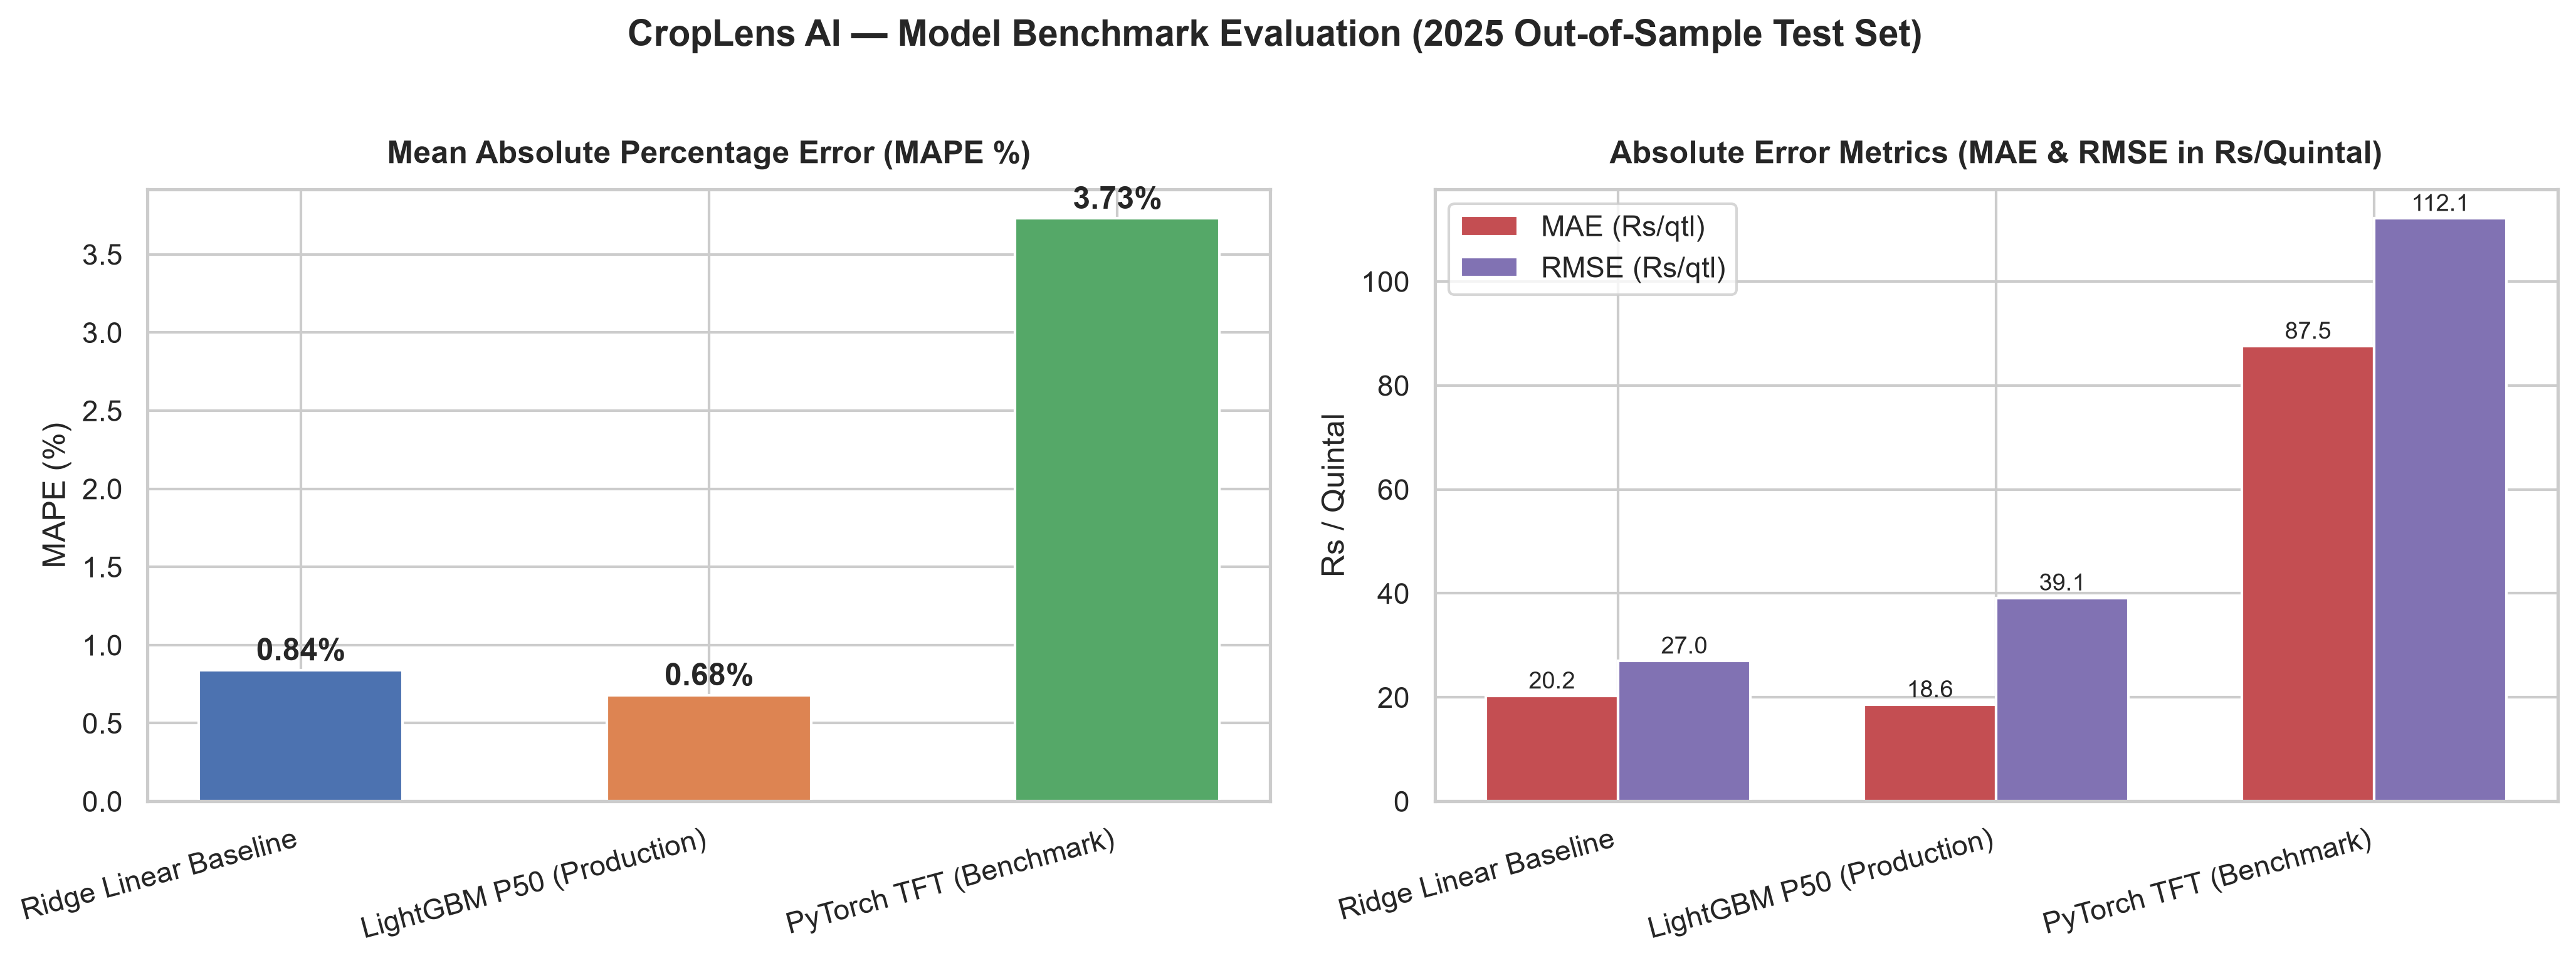
\includegraphics[width=\columnwidth]{figures/8_model_benchmark_comparison.png}
\caption{Model benchmark comparison on the frozen 2025 test scope.}
\label{fig:benchmark}
\end{figure}

\subsection{Uncertainty Calibration and Quantile Validity}
Table~\ref{tab:uncertainty} summarises the behaviour of the P10--P90 interval. Before applying CQR, empirical coverage is 76.69\% with an average interval width (MPIW) of INR~222.22/qtl. Adding the global CQR offset widens the band modestly to MPIW INR~228.78/qtl and raises coverage to 79.49\%, close to the 80\% nominal target. On the 2025 test set 652 of 19{,}240 raw triplets contain a crossing; rearrangement reduces the post-processing crossing count to zero. This ordering step is separate from calibration: rearrangement only enforces P10 $\le$ P50 $\le$ P90, while CQR adjusts the width based on validation residuals.

\begin{table}[t]
\caption{Frozen P10--P90 uncertainty results on the 2025 holdout}
\label{tab:uncertainty}
\centering
\small
\begin{tabular}{@{}lrr@{}}
\toprule
Quantity & Uncalibrated & CQR \\
\midrule
Nominal coverage (\%) & 80.00 & 80.00 \\
Empirical coverage (\%) & 76.69 & 79.49 \\
MPIW (INR/qtl) & 222.22 & 228.78 \\
Raw crossings (of 19{,}240) & 652 & 652 \\
Post-rearrangement crossings & 0 & 0 \\
\bottomrule
\end{tabular}
\end{table}

\begin{figure}[t]
\centering
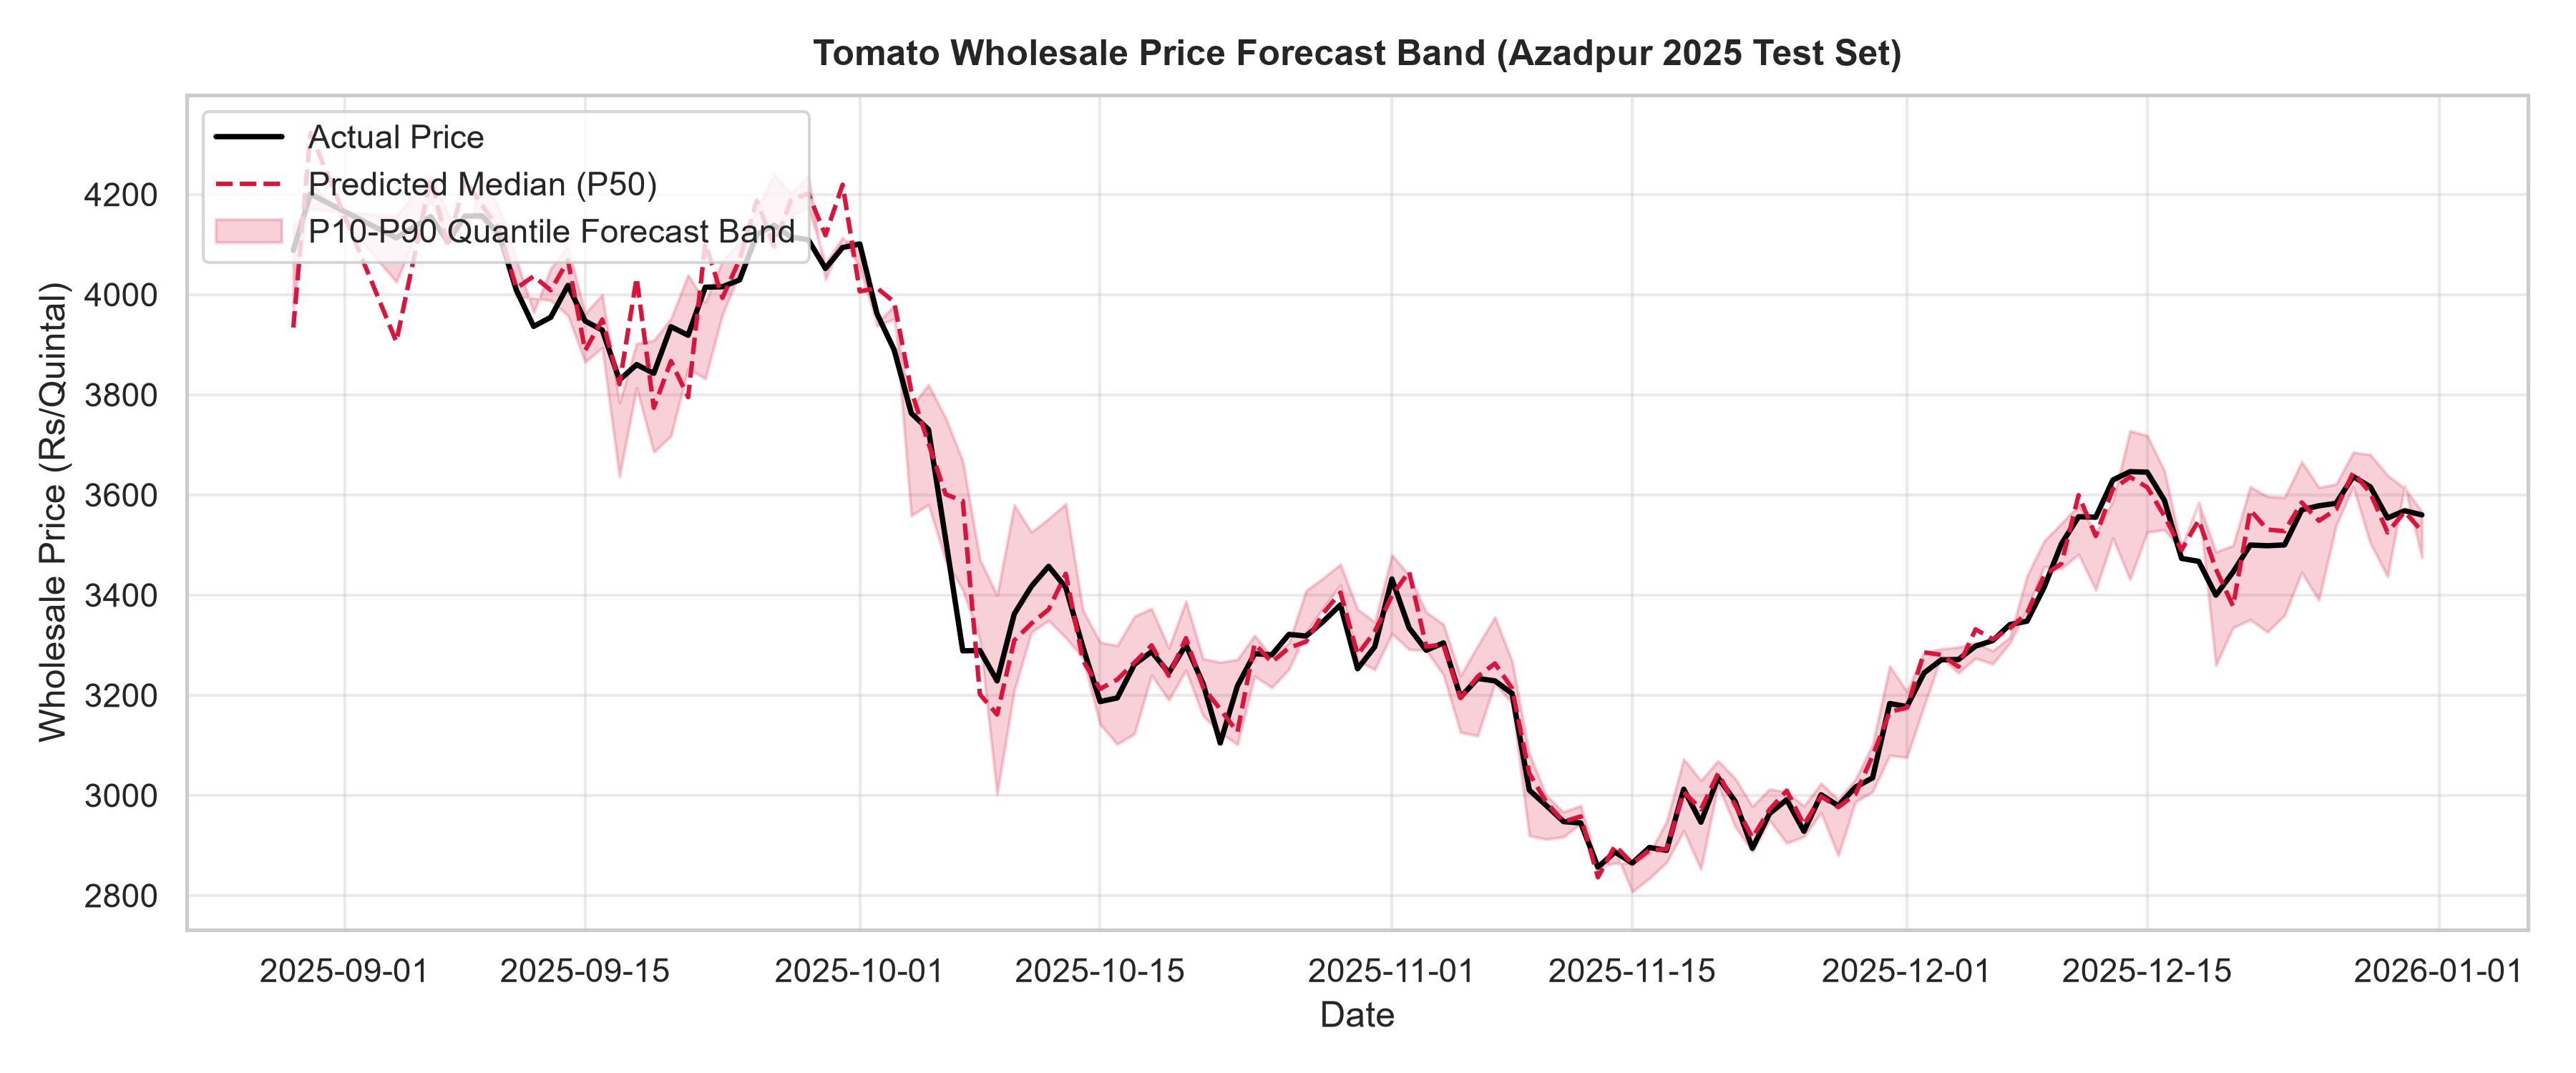
\includegraphics[width=\columnwidth]{figures/6_prediction_intervals_p10_p90.png}
\caption{Calibrated P10--P90 prediction intervals and realized prices for a representative commodity--mandi series in 2025. The band captures most outcomes while still exposing large downside and upside moves.}
\label{fig:intervals}
\end{figure}

\subsection{Ablation and Market-Group Behaviour}
Feature ablations confirm that price history is the dominant signal. Dropping price lags and momentum lifts LightGBM P50 MAE from INR~82.00/qtl to about INR~116.76/qtl and pushes MAPE from 1.28\% to 1.85\%. Removing arrivals alone has a smaller effect (MAE $\approx$ INR~83.36/qtl), as does removing festival features (MAE $\approx$ INR~81.96/qtl). Weather and NDVI variables contribute complementary information rather than dominating on their own. Commodity-level errors are uneven: MAE is around INR~17--20/qtl for Maize, Paddy, Wheat, and Potato, but exceeds INR~500/qtl for Chilli Red. That pattern matches field intuition about highly volatile spice and cash-crop series. Table~\ref{tab:easy_hard_groups} contrasts two relatively easier commodities (Maize, Wheat) with two harder ones (Chilli Red, Mustard) under the LightGBM P50 vs naive persistence comparison.

\begin{table}[t]
\caption{Example easy and hard commodity groups on the 2025 holdout (LightGBM P50 vs naive persistence). Errors are in INR per quintal.}
\label{tab:easy_hard_groups}
\centering
\small
\begin{tabular}{@{}lrrr@{}}
\toprule
Commodity & Test rows & Naive MAE & LGBM MAE \\
\midrule
Maize & 2{,}184 & 22.18 & 17.22 \\
Wheat & 2{,}184 & 19.52 & 17.33 \\
Chilli Red & 1{,}456 & 355.32 & 511.36 \\
Mustard & 1{,}820 & 71.18 & 114.71 \\
\bottomrule
\end{tabular}
\end{table}

\subsection{Statistical Tests and Residual Diagnostics}
Diebold--Mariano tests under absolute-error loss indicate that Ridge is significantly better than LightGBM P50 on MAE and MAPE (Newey--West $p < 0.001$), and that LightGBM modestly improves over XGBoost on MAE while being similar under squared loss. Comparisons with CatBoost depend on the chosen loss function. Ljung--Box diagnostics on validation residuals reveal significant autocorrelation at lags 7, 14, and 30 across many series ($p < 0.001$), which points to weekly auction cycles and unmodelled seasonal or policy effects that are not yet captured by the feature set. High $R^2$ values therefore should not be interpreted as evidence that the dynamics are fully explained.

\subsection{Operational Anomaly Triage}
Isolation Forest is trained as an unsupervised filter on arrival ratio, arrival velocity, price volatility, and spread. On the 2025 test set it flags 1{,}283 of 19{,}240 observations (6.67\%) as potential anomalies. When compared with proxy rules based on high arrival ratio ($>1.5$) or steep negative price velocity ($<-50$ INR/qtl/day), the system attains around 96.0\% specificity and proxy precision and recall in the low-40\% range. These numbers describe agreement with a hand-crafted heuristic rather than supervised classification accuracy. In use, a flagged day is intended to prompt an analyst to look more closely at the series, not to certify that a supply shock definitely occurred.

\subsection{Fairness, Spatial Transfer, and Interpretability}
LOMO experiments indicate good transfer for some mandis (for example, Khanna with MAE $\approx$ INR~15.14/qtl) but substantial degradation for others such as Azadpur (MAE $\approx$ INR~276.53/qtl) and Kolkata. This heterogeneity means that fairness, in the sense of similar error levels across markets and crops, cannot be assumed even with a shared training pipeline. TreeSHAP explanations highlight short-term price lags and volatility as the dominant features, with modest contributions from arrivals, NDVI momentum, and spatial gradients \cite{lundberg2020local}. Granger tests suggest predictive association for several exogenous variables \cite{granger1969investigating}, but we treat these results as descriptive and avoid causal language.

\section{Operational Integration}
The production loader requires a complete model bundle: three quantile estimators, feature metadata, target declaration, feature ordering, and version identifiers. It refuses to load a partial bundle as a production model. Service initialisation also checks that the serving dataset is non-empty, has valid dates, and contains all required model columns. Online data synchronisation with Agmarknet, NASA POWER, and Sentinel-2 does not fabricate missing values: incomplete live rows are skipped and logged, and cache initialisation proceeds only when both models and serving data are available. This conservative behaviour means that a good offline metric is not enough; the service must also show that it can load the certified package and ingest live data without entering a failure-safe state.

Reproducibility is treated here as a property of a concrete evidence bundle rather than just of the narrative text. In our case, that bundle consists of a frozen experiment manifest, the canonical benchmark and uncertainty metrics, the bootstrap summaries, the per-commodity and per-mandi breakdowns, and a claim--evidence matrix that links specific sentences in the paper to specific runs and artefacts. The manifest records the dataset scope, date range, splits, commodity and mandi lists, feature count, target variable, forecast horizon, random seed, and evaluation rules. The mapping then indicates which tables, plots, or CSV files back up a given statement. This structure is intended to make it harder to overinterpret a convenient number outside its documented scope, and to give a future reviewer enough information to re-run or extend the analysis.

In practice we treat the model and dataset as certified only when a small set of checks passes; Table~\ref{tab:certification} summarises the most important ones.

\begin{table}[t]
\caption{Key certification controls in the production pipeline}
\label{tab:certification}
\centering
\small
\begin{tabular}{@{}p{0.32\columnwidth}p{0.58\columnwidth}@{}}
\toprule
Control & Intended protection \\
\midrule
Target signature & Confirms that the model predicts next-day modal price rather than a shifted or contemporaneous value. \\
Feature signature & Checks that the 47 feature names, order, and count match between training and serving. \\
Temporal signature & Verifies the 2019--2023 training, 2024 validation, and 2025 test protocol. \\
Bundle completeness & Prevents loading a bundle with only one or two quantiles as a production model. \\
Checkpoint signature & Avoids mixing incompatible model packages when resuming training from intermediate stages. \\
Live-row validation & Skips incomplete upstream observations instead of fabricating weather, NDVI, or market values. \\
Evidence freeze & Ensures that reported metrics are copied from a single dated evaluation record rather than recomputed ad hoc. \\
\bottomrule
\end{tabular}
\end{table}

\section{Limitations and Future Work}
The results come with several caveats that matter for how the system should be used. Ridge and ARIMA achieve lower aggregate point error than the quantile LightGBM system; the production model is justified by its P10--P90 bands and operational integration, not by winning every point metric. Modal prices are highly persistent, so naive and linear baselines are strong and define a realistic performance floor. Residual autocorrelation at weekly and monthly lags shows that important structure is still missing from the feature set or model class. Errors are much larger for commodities such as Chilli Red and for terminal markets such as Azadpur, so transfer across crops and mandis is not uniform. LSTM, GRU, and TFT are proof-of-concept runs that were not tuned as aggressively as the tree models, and Isolation Forest is evaluated only against proxy rules. COVID-era behaviour is examined in-sample, not as an unseen stress test. Finally, CQR calibration is based on historical validation data; under distribution shift the nominal 80\% coverage target may not hold even if the feature contract stays fixed.

Future work could therefore move in several directions: stronger probabilistic sequence baselines with richer covariates and tuning; hierarchical or multi-level models across commodities and mandis; external-market validation; explicit checks for distribution shift and dynamic recalibration of intervals; and anomaly evaluation against curated event labels instead of heuristics.

\section{Conclusion}
CropLens AI puts together a leakage-aware framework for next-day APMC price forecasting rather than a single model in isolation. The core design choices are a fixed next-day modal-price target, a 47-feature contract that is shared between training and serving, and strict chronological splits with a frozen 2025 holdout. On top of this, a three-quantile LightGBM model, rearrangement, and validation-only CQR produce ordered P10--P90 bands that reach 79.49\% empirical coverage on the test set, while Ridge and ARIMA still lead on aggregate point error.

The empirical analysis shows that the pipeline is most reliable for some staple crops and interior mandis, and much weaker for volatile commodities and busy terminal markets. Residual tests and anomaly diagnostics emphasise that important structure is still missing and that shocks cannot yet be treated as fully labelled events. Taken together, the results support using CropLens AI as a decision-support system that surfaces both central forecasts and risk bands, and that is honest about where errors remain high, rather than as a claim of universal model superiority or complete supply-shock detection.

\section*{Acknowledgment}
The authors thank their mentors and faculty for guidance on agricultural data analysis, machine learning evaluation, software engineering, and scientific communication.

\bibliographystyle{IEEEtran}
\bibliography{references}
\end{document}